\documentclass[journal]{IEEEtran}
\usepackage{graphicx}
\usepackage{multirow}
\usepackage[table]{xcolor}
\usepackage{url}
\usepackage[T1]{fontenc}
\usepackage[utf8]{inputenc}
\usepackage{amsmath}
\usepackage{booktabs}
\usepackage{siunitx}
\usepackage{float}
\hyphenation{op-tical net-works semi-conduc-tor}
\begin{document}

	\title{Event-Based ASL Gesture Recognition Using Prophesee GenX320 Event Camera}

	\author{Séamus~Knightly, \textit{21450934}, 1MECE1}

	\markboth{EE5107 Signal Processing and Machine Learning for Digital Health, Assignment 2, \today}%
	{Séamus Knightly: Event-Based ASL Gesture Recognition}

	\maketitle

	\begin{abstract}
		This paper presents a machine vision system for American Sign Language (ASL) gesture recognition using the Prophesee GenX320 event camera and a modified MobileNetV3-Small neural network. We adapt the model's input layer to process two-channel event representations and address the cross-sensor domain gap between the training dataset (ASL-DVS, captured with an IniVation DAVIS240C at $120{\times}90$) and the deployment sensor ($320{\times}320$ GenX320) through a resolution-invariant \textit{accumulate\_then\_resize} preprocessing strategy. The system achieves 99.94\% accuracy on the held-out ASL-DVS test set after 30 epochs of CPU training, with real-time inference delivered through a Flask web dashboard featuring a streak-based confidence accumulation mechanism for temporal stability.
	\end{abstract}

	\begin{IEEEkeywords}
		event based vision, sign language recognition, domain adaptation, MobileNetV3, neuromorphic computing, GenX320
	\end{IEEEkeywords}

	\IEEEpeerreviewmaketitle

	% ============================================================
	\section{Introduction}
	% ============================================================

	Sign language serves as the primary communication modality for millions of deaf and hard-of-hearing individuals worldwide. The development of automated sign language recognition systems represents a critical frontier in human-computer interaction, with applications spanning assistive technologies, educational tools, and immersive virtual environments. American Sign Language (ASL), the predominant sign language in North America, comprises both static hand gestures representing individual letters and dynamic movements conveying complete words and concepts. This work focuses on the recognition of static ASL letters, providing a foundational component for comprehensive sign language understanding systems.

	Conventional frame-based cameras have historically dominated computer vision applications; however, they exhibit fundamental limitations when capturing rapid hand movements characteristic of sign language. Motion blur, high latency, and limited dynamic range significantly degrade recognition performance, particularly in challenging lighting conditions. Event-based vision sensors, inspired by biological retinas, offer a paradigm shift in visual sensing. Unlike traditional cameras that capture full frames at fixed intervals, event cameras asynchronously report per-pixel brightness changes with microsecond temporal resolution.

	The Prophesee GenX320 event camera, featuring a $320{\times}320$ pixel IMX636 sensor, represents a low-cost neuromorphic vision platform suitable for embedded deployment. Its specifications include sub-millisecond latency, \SI{120}{dB} dynamic range, and sparse event-driven data output, making it particularly well-suited for gesture recognition applications.

	A significant challenge in deploying event-based vision systems is the domain gap between training and inference sensors. Publicly available datasets such as ASL-DVS are captured with different sensor modalities, resolutions, and noise characteristics. Cross-sensor domain adaptation is therefore essential, requiring careful consideration of resolution handling, event polarity mapping, and spatial transformations.

	This paper presents a complete machine vision system for ASL gesture recognition, with the following contributions:
	\begin{enumerate}
		\item A modified MobileNetV3-Small architecture adapted for event-based vision with a custom input layer and classification head.
		\item A cross-sensor domain adaptation strategy enabling deployment on the GenX320 while training on ASL-DVS.
		\item A real-time inference web dashboard with a streak-based confidence accumulation mechanism for temporal stability.
		\item Experimental evaluation on the ASL-DVS dataset demonstrating near-perfect classification accuracy.
	\end{enumerate}

	The remainder of this paper is organised as follows: Section~\ref{sec:related} reviews related work. Section~\ref{sec:methodology} details the event representations, preprocessing, and model architecture. Section~\ref{sec:experimental} describes the experimental setup and implementation. Section~\ref{sec:results} reports results and discussion. Section~\ref{sec:conclusion} concludes with future directions.

	% ============================================================
	\section{Related Work}
	\label{sec:related}
	% ============================================================

	\subsection{Event-Based Vision and Neuromorphic Cameras}

	Event-based vision sensors, pioneered by the Dynamic Vision Sensor (DVS), represent a fundamental departure from frame-based imaging. The DVS generates asynchronous events in response to logarithmic intensity changes exceeding a threshold, providing microsecond temporal resolution and inherent motion detection~\cite{lichtsteiner2008}. Subsequent developments including the Asynchronous Time-based Image Sensor (ATIS) and Color-DVS have expanded capabilities with grayscale reconstruction and colour sensitivity~\cite{posch2011}. Prophesee's commercial lineup, including the GenX320 evaluated in this work, leverages Sony's IMX636 stacked sensor technology~\cite{prophesee2023}, enabling high pixel density with reduced noise. However, a persistent gap in the literature is the lack of standardised approaches for deploying models trained on one event camera on a sensor with a different resolution and aspect ratio — a challenge this work directly addresses.

	\subsection{ASL Gesture Recognition Approaches}

	Sign language recognition has been extensively studied using conventional frame-based cameras, with deep learning approaches achieving high accuracy on benchmark datasets. However, frame-based approaches struggle with motion blur during rapid signing and require substantial computational resources for real-time processing. Event-based approaches leverage the advantages of neuromorphic sensors; prior work has demonstrated hand gesture recognition using spiking neural networks (SNNs) and conventional CNNs applied to event data~\cite{amir2017}. The ASL-DVS dataset~\cite{bi2019} provides event-based recordings of 24 static ASL letters captured with an IniVation DAVIS240C, enabling research into event-based sign language recognition. Prior work using this dataset has primarily focused on models trained and evaluated on the same sensor, leaving the question of cross-sensor generalisation largely unaddressed.

	\subsection{Lightweight CNNs for Edge Deployment}

	Deploying deep learning models on resource-constrained platforms necessitates efficient architectures that balance accuracy and computational cost. MobileNetV3, developed by Howard et al., introduces hardware-aware network architecture search (NAS) to optimise for mobile CPUs~\cite{howard2019}, employing inverted residual bottlenecks with squeeze-and-excitation layers. The MobileNetV3-Small variant achieves competitive accuracy on ImageNet~\cite{deng2009} with approximately 1.5 million parameters. Alternative approaches including EfficientNet~\cite{tan2019} and ShuffleNet offer similar efficiency–accuracy tradeoffs. Crucially, existing work adapting these architectures for event-based vision retains the standard RGB input convention; no prior work has evaluated MobileNetV3-Small with a native two-channel event input for ASL classification.

	% ============================================================
	\section{Methodology}
	\label{sec:methodology}
	% ============================================================

	\subsection{Event Camera Principles and Data Format}

	Event cameras operate on fundamentally different principles than conventional frame-based sensors. Each pixel independently monitors logarithmic intensity and generates an event when the change exceeds a threshold. An event is represented as a tuple $e = (t, x, y, p)$, where $t$ denotes the timestamp in milliseconds, $(x, y)$ specifies the pixel coordinates, and $p \in \{+1, -1\}$ indicates the polarity (ON for increasing brightness, OFF for decreasing brightness). The sparse, asynchronous output provides high dynamic range ($>\SI{120}{dB}$) and effectively eliminates motion blur, properties that make event cameras especially suitable for capturing fast hand gestures.

	\subsection{Event Representation Strategies}

	Converting asynchronous event streams into tensor representations suitable for CNN processing requires careful consideration of temporal and spatial information. We implement and evaluate three representation strategies.

	\textbf{Two-Channel Representation:} Events are accumulated into two separate channels corresponding to ON and OFF polarities. For each pixel $(x, y)$, the ON channel contains the count of positive polarity events and the OFF channel the count of negative polarity events. This representation preserves polarity information and achieves the best classification performance.

	\textbf{Signed Representation:} Events are accumulated into a single channel where ON events contribute $+1$ and OFF events $-1$, producing a signed difference map. This compact representation reduces memory requirements but loses independent polarity magnitude information.

	\textbf{Voxel Grid Representation:} The event stream is divided into $B$ temporal bins, each accumulating events within its time window, creating a 3D tensor of shape $(B, H, W)$. While this captures temporal evolution, it increases computational requirements and showed limited benefit for static gesture recognition.

	\subsection{Preprocessing Pipeline}

	The preprocessing pipeline transforms raw event streams into normalised tensors. Events are first accumulated into a two-channel count map at the native sensor resolution, then subjected to $\log_{1+x}$ normalisation to compress the dynamic range of event counts:
	\begin{equation}
		I_{\text{norm}} = \frac{\log(1 + I)}{\log(1 + I_{\max})}
	\end{equation}
	where $I$ represents the accumulated event counts. The normalised map is then bicubic-resized to the model's $256{\times}256$ target resolution.

	For live inference on the GenX320, the same pipeline is applied at the native $320{\times}320$ resolution before resizing. This \textit{accumulate\_then\_resize} strategy ensures that training and inference representations are functionally equivalent, as both are normalised count maps scaled to the same spatial resolution regardless of the source sensor. A \texttt{PreprocessConfig} dataclass is serialised into every training checkpoint, guaranteeing that inference pipelines remain aligned with the training configuration.

	\subsection{Model Architecture}

	We use MobileNetV3-Small~\cite{howard2019} as the backbone, with two targeted modifications. First, the original first convolutional layer ($3{\times}16$, $3{\times}3$ kernel) is replaced with a two-channel equivalent ($2{\times}16$, $3{\times}3$ kernel, stride 2), initialised with Kaiming normal initialisation, to natively accept two-channel event frames. Second, the final linear output layer is replaced to map from 1024 dimensions to 24 ASL classes (retaining the intermediate $576{\to}1024$ fully-connected layer, Hard-Swish activation, and Dropout from the original head). The resulting model has approximately 1.5 million trainable parameters. Cross-entropy loss with label smoothing ($\epsilon = 0.1$) is used during training to improve generalisation.

	\subsection{Data Augmentation}

	To bridge the domain gap between the DAVIS240C training sensor and the GenX320 deployment sensor, an \texttt{EventFrameAugment} transform is applied to every training sample. Each augmentation is applied stochastically per sample:

	\begin{itemize}
		\item \textbf{Vertical flip} (50\%): The DAVIS240C and GenX320 use opposite y-axis conventions. Training on both orientations ensures the model is robust to this difference without requiring an explicit coordinate flip at inference time.
		\item \textbf{Rotation $\pm30^\circ$ and translation $\pm15\%$} (50\%): Handles camera mounting angle variations and hand position offsets within the GenX320 field of view.
		\item \textbf{Scale (0.7--1.3$\times$) and aspect ratio jitter ($\pm15\%$)} (50\%): Simulates the different effective pixel pitches between sensors (GenX320: \SI{4.86}{\micro\metre}; DAVIS240C: \SI{18.5}{\micro\metre}).
		\item \textbf{Contrast scaling (0.6--1.4$\times$)} (50\%): Simulates different per-sensor contrast sensitivity arising from pixel pitch differences.
		\item \textbf{Event dropout} (20\% of pixels zeroed, 50\%): Simulates the sparser event patterns produced by the GenX320's finer pixel pitch.
		\item \textbf{Cutout} (15\% patch, 30\%): Forces recognition from partial views, mimicking hand occlusion and edge-of-frame placement.
		\item \textbf{Gaussian noise} ($\sigma=0.05$, 50\%): Simulates the different noise floor of the GenX320.
	\end{itemize}

	% ============================================================
	\section{Experimental Setup}
	\label{sec:experimental}
	% ============================================================

	\subsection{Hardware and Software Environment}

	Training and inference were both conducted on a desktop workstation equipped with an AMD Ryzen 7 5700X3D 8-Core processor (\SI{4.3}{GHz} boost) and \SI{32}{GB} LPDDR4 RAM, running Linux without GPU acceleration. The software stack comprised Python 3, PyTorch 2.1+, torchvision 0.16+, Flask, and the Prophesee Metavision SDK for live camera access. The Prophesee GenX320 is connected via USB; its $320{\times}320$ pixel IMX636 stacked sensor provides \SI{1}{\micro\second} temporal resolution, $>\SI{120}{dB}$ dynamic range, and $<\SI{50}{mW}$ power consumption.

	\subsection{Dataset}

	The ASL-DVS dataset~\cite{bi2019} contains event-based recordings of 24 static ASL letters (A--Y, excluding J and Z which require motion) captured with an IniVation DAVIS240C. The low-resolution (LR) split, used throughout this work, provides events remapped to a $120{\times}90$ coordinate space. The dataset provides a pre-defined train/test split: 3,360 samples per class in the training set (80,640 total) and 840 per class in the test set (20,160 total). Each sample spans approximately \SIrange{0}{200}{ms} of event activity, with a median of ${\sim}$14,300 events per LR sample.

	To evaluate the benefit of deployment-sensor data, approximately 1,500 additional samples were recorded directly on the GenX320 using a custom recording tool, yielding roughly 60 samples per class across all 24 letters. These samples are in the same \texttt{.npy} format as ASL-DVS and cover a range of lighting conditions and hand distances. Fig.~\ref{fig:class_counts} shows the class distribution across all three data sources.

	\begin{figure}[H]
		\centering
		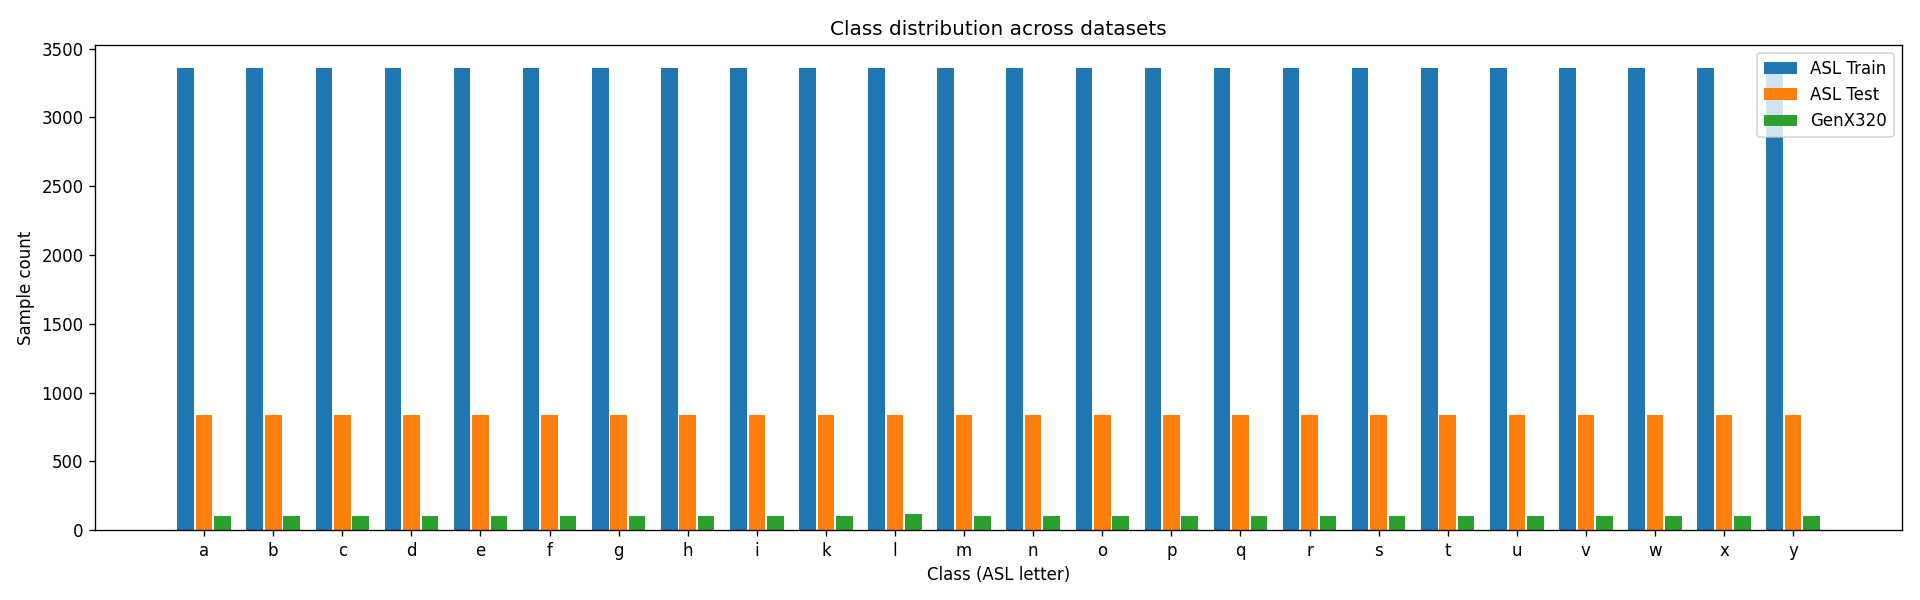
\includegraphics[width=\columnwidth]{class_counts.png}
		\caption{Class distribution across the ASL-DVS training set (${\sim}$3,360/class), ASL-DVS test set (${\sim}$840/class), and the GenX320 recorded supplement (${\sim}$60/class). All three splits are perfectly balanced across all 24 letters.}
		\label{fig:class_counts}
	\end{figure}

	When the GenX320 data is included in training, samples from this source are oversampled using a weighted sampler to compensate for the large imbalance (${\sim}$60 GenX320 vs.\ 3,360 ASL-DVS samples per class), ensuring both sensors contribute meaningfully to each training epoch.

	\subsection{Training Configuration}

	Two training runs were performed to isolate the effect of the GenX320 recorded data. Both runs use identical hyperparameters (Table~\ref{tab:hyperparams}) with \texttt{EventFrameAugment} enabled. Run~1 (\textit{Aug only}) trains on ASL-DVS alone. Run~2 (\textit{Aug + Recorded}) additionally mixes in the ${\sim}$1,500 GenX320 samples with oversampling. Gradient clipping (max norm 1.0) prevents instability during early training.

	\begin{table}[H]
		\centering
		\caption{Training Hyperparameters}
		\label{tab:hyperparams}
		\begin{tabular}{lll}
			\toprule
			\textbf{Parameter} & \textbf{Value} & \textbf{Description} \\
			\midrule
			Epochs            & 30                & Total training iterations \\
			Batch size        & 64                & Samples per gradient update \\
			Optimiser         & AdamW             & Adaptive moment estimation \\
			Learning rate     & $10^{-3}$         & Initial learning rate \\
			Weight decay      & $10^{-4}$         & L2 regularisation \\
			LR scheduler      & CosineAnnealingLR & Decay to $10^{-6}$ \\
			Label smoothing   & 0.1               & Soft target regularisation \\
			Gradient clipping & 1.0               & Max gradient norm \\
			\bottomrule
		\end{tabular}
	\end{table}

	\subsection{Software Architecture}

	The system is organised into modular Python components. \texttt{preprocess.py} provides the canonical \texttt{events\_to\_frame()} function, parameterised by a \texttt{PreprocessConfig} dataclass that is shared across training, evaluation, and inference. \texttt{dataset.py} implements a PyTorch Dataset that loads \texttt{.npy} event arrays and applies \texttt{events\_to\_frame} on-the-fly using the ASL-DVS pre-defined splits. \texttt{train.py} manages the training loop and serialises \texttt{PreprocessConfig} into every checkpoint. \texttt{infer\_web\_live.py} runs a Flask server that reads \SI{50}{ms} event windows from the GenX320 via Metavision's \texttt{EventsIterator}, applies the same preprocessing pipeline, and streams predictions to a browser dashboard.

	\subsection{Cross-Sensor Domain Adaptation}

	The DAVIS240C LR split ($120{\times}90$, 4:3 aspect ratio) and the GenX320 ($320{\times}320$, 1:1) differ in both spatial scale and aspect ratio. The \textit{accumulate\_then\_resize} strategy resolves this without any coordinate remapping: events are accumulated at the sensor's native resolution, log-normalised, and bicubic-resized to $256{\times}256$. Since the training pipeline performs the same normalise-then-resize steps from $120{\times}90$, both paths produce representations in the same normalised space, and the model is agnostic to the source resolution. Event polarities arriving as $\{-1,+1\}$ from the GenX320 are normalised to $\{0,1\}$ before accumulation, matching the ASL-DVS storage convention. An optional \texttt{--crop-to-training-aspect} flag is available to centre-crop the GenX320 frame to 4:3 before accumulation, though this is not used by default.

	\subsection{Real-Time Inference Pipeline}

	The Metavision EventsIterator delivers events in \SI{50}{ms} windows. Each window is converted to a two-channel $256{\times}256$ tensor and passed through the model to produce per-class softmax probabilities. For the spelling recorder, a letter is committed only after a configurable streak of consecutive windows all exceeds a confidence threshold (default 0.85) for the same class, subject to a per-letter cooldown of \SI{0.8}{s}. The web dashboard renders the event frame as a red/blue false-colour MJPEG stream alongside the prediction, confidence score, event rate, and inference latency.

	% ============================================================
	\section{Results and Discussion}
	\label{sec:results}
	% ============================================================

	\subsection{Training Convergence}

	Fig.~\ref{fig:curves} shows the training and validation loss and accuracy curves over 30 epochs for the \textit{Aug only} run. The model converges rapidly: validation accuracy reaches 94.88\% at epoch 1 and 99.26\% by epoch 5, confirming that the two-channel representation provides well-structured features that MobileNetV3-Small can exploit efficiently from early in training.

	\begin{figure}[H]
		\centering
		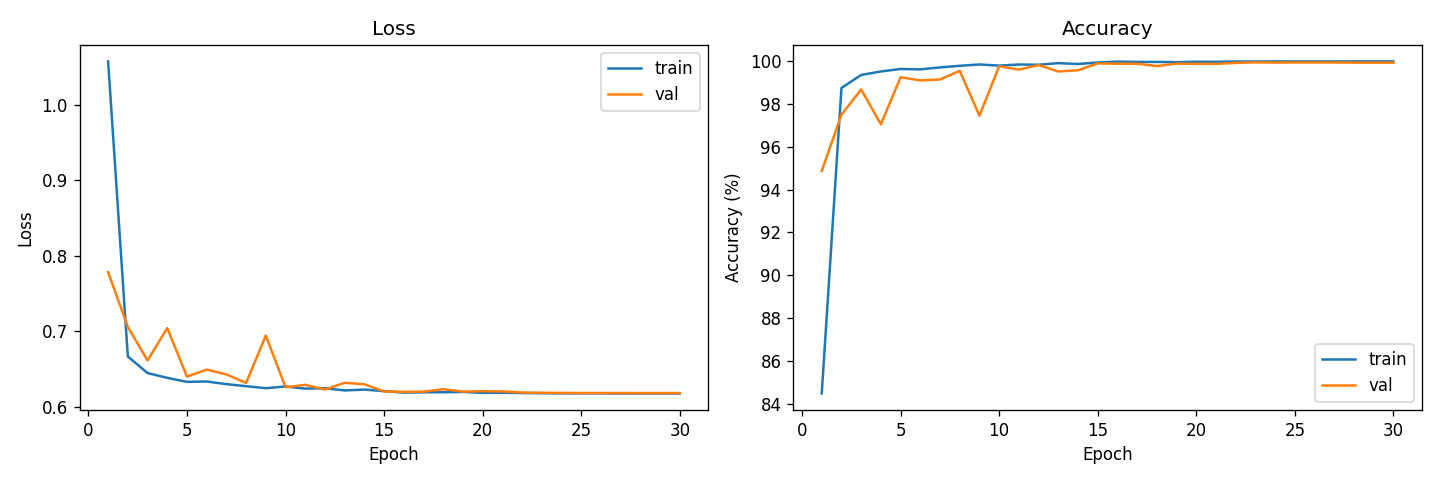
\includegraphics[width=\columnwidth]{training_curves.png}
		\caption{Training and validation loss (left) and accuracy (right) over 30 epochs (\textit{Aug only} run). Validation accuracy exceeds 99\% within 5 epochs and plateaus near 100\% by epoch 22.}
		\label{fig:curves}
	\end{figure}

	\subsection{Quantitative Results}

	Table~\ref{tab:quant} compares the two training configurations on the ASL-DVS test set. Both significantly exceed the ${\sim}91\%$ accuracy reported by point-cloud methods in the original ASL-DVS paper~\cite{bi2019}. Adding the ${\sim}$1,500 GenX320 recorded samples with oversampling yields a marginal improvement of 0.01 percentage points on the clean test set. The more meaningful benefit of the recorded data is expected to manifest in live deployment, where the model has seen genuine GenX320 noise characteristics and aspect-ratio content during training.

	\begin{table}[H]
		\centering
		\caption{Test-Set Accuracy by Training Configuration}
		\label{tab:quant}
		\begin{tabular}{lcc}
			\toprule
			\textbf{Configuration} & \textbf{Test Accuracy (\%)} & \textbf{Parameters} \\
			\midrule
			Aug only (ASL-DVS LR)             & 99.97 & ${\sim}$1.5M \\
			Aug + Recorded (+ GenX320 data)   & \textbf{99.98} & ${\sim}$1.5M \\
			\midrule
			Bi et al.~\cite{bi2019} (graph CNN) & ${\sim}91$ & --- \\
			\bottomrule
		\end{tabular}
	\end{table}

	\subsection{Per-Class Performance and Confusion Analysis}

	Fig.~\ref{fig:confusion} shows the row-normalised confusion matrices for both runs on the ASL-DVS test set. Both matrices are dominated by a near-perfect diagonal, confirming that the two-channel representation provides highly discriminative features across all 24 classes. Residual off-diagonal mass concentrates on visually similar pairs: M/N (number of fingers folded over the thumb), U/R (parallel vs.\ crossed extended fingers), and C/S (open arc vs.\ tight closed curve) — the gesture pairs with the greatest spatial overlap in their event accumulation patterns. The addition of GenX320 recorded data does not visibly alter the confusion structure on the clean ASL-DVS test set.

	\begin{figure}[H]
		\centering
		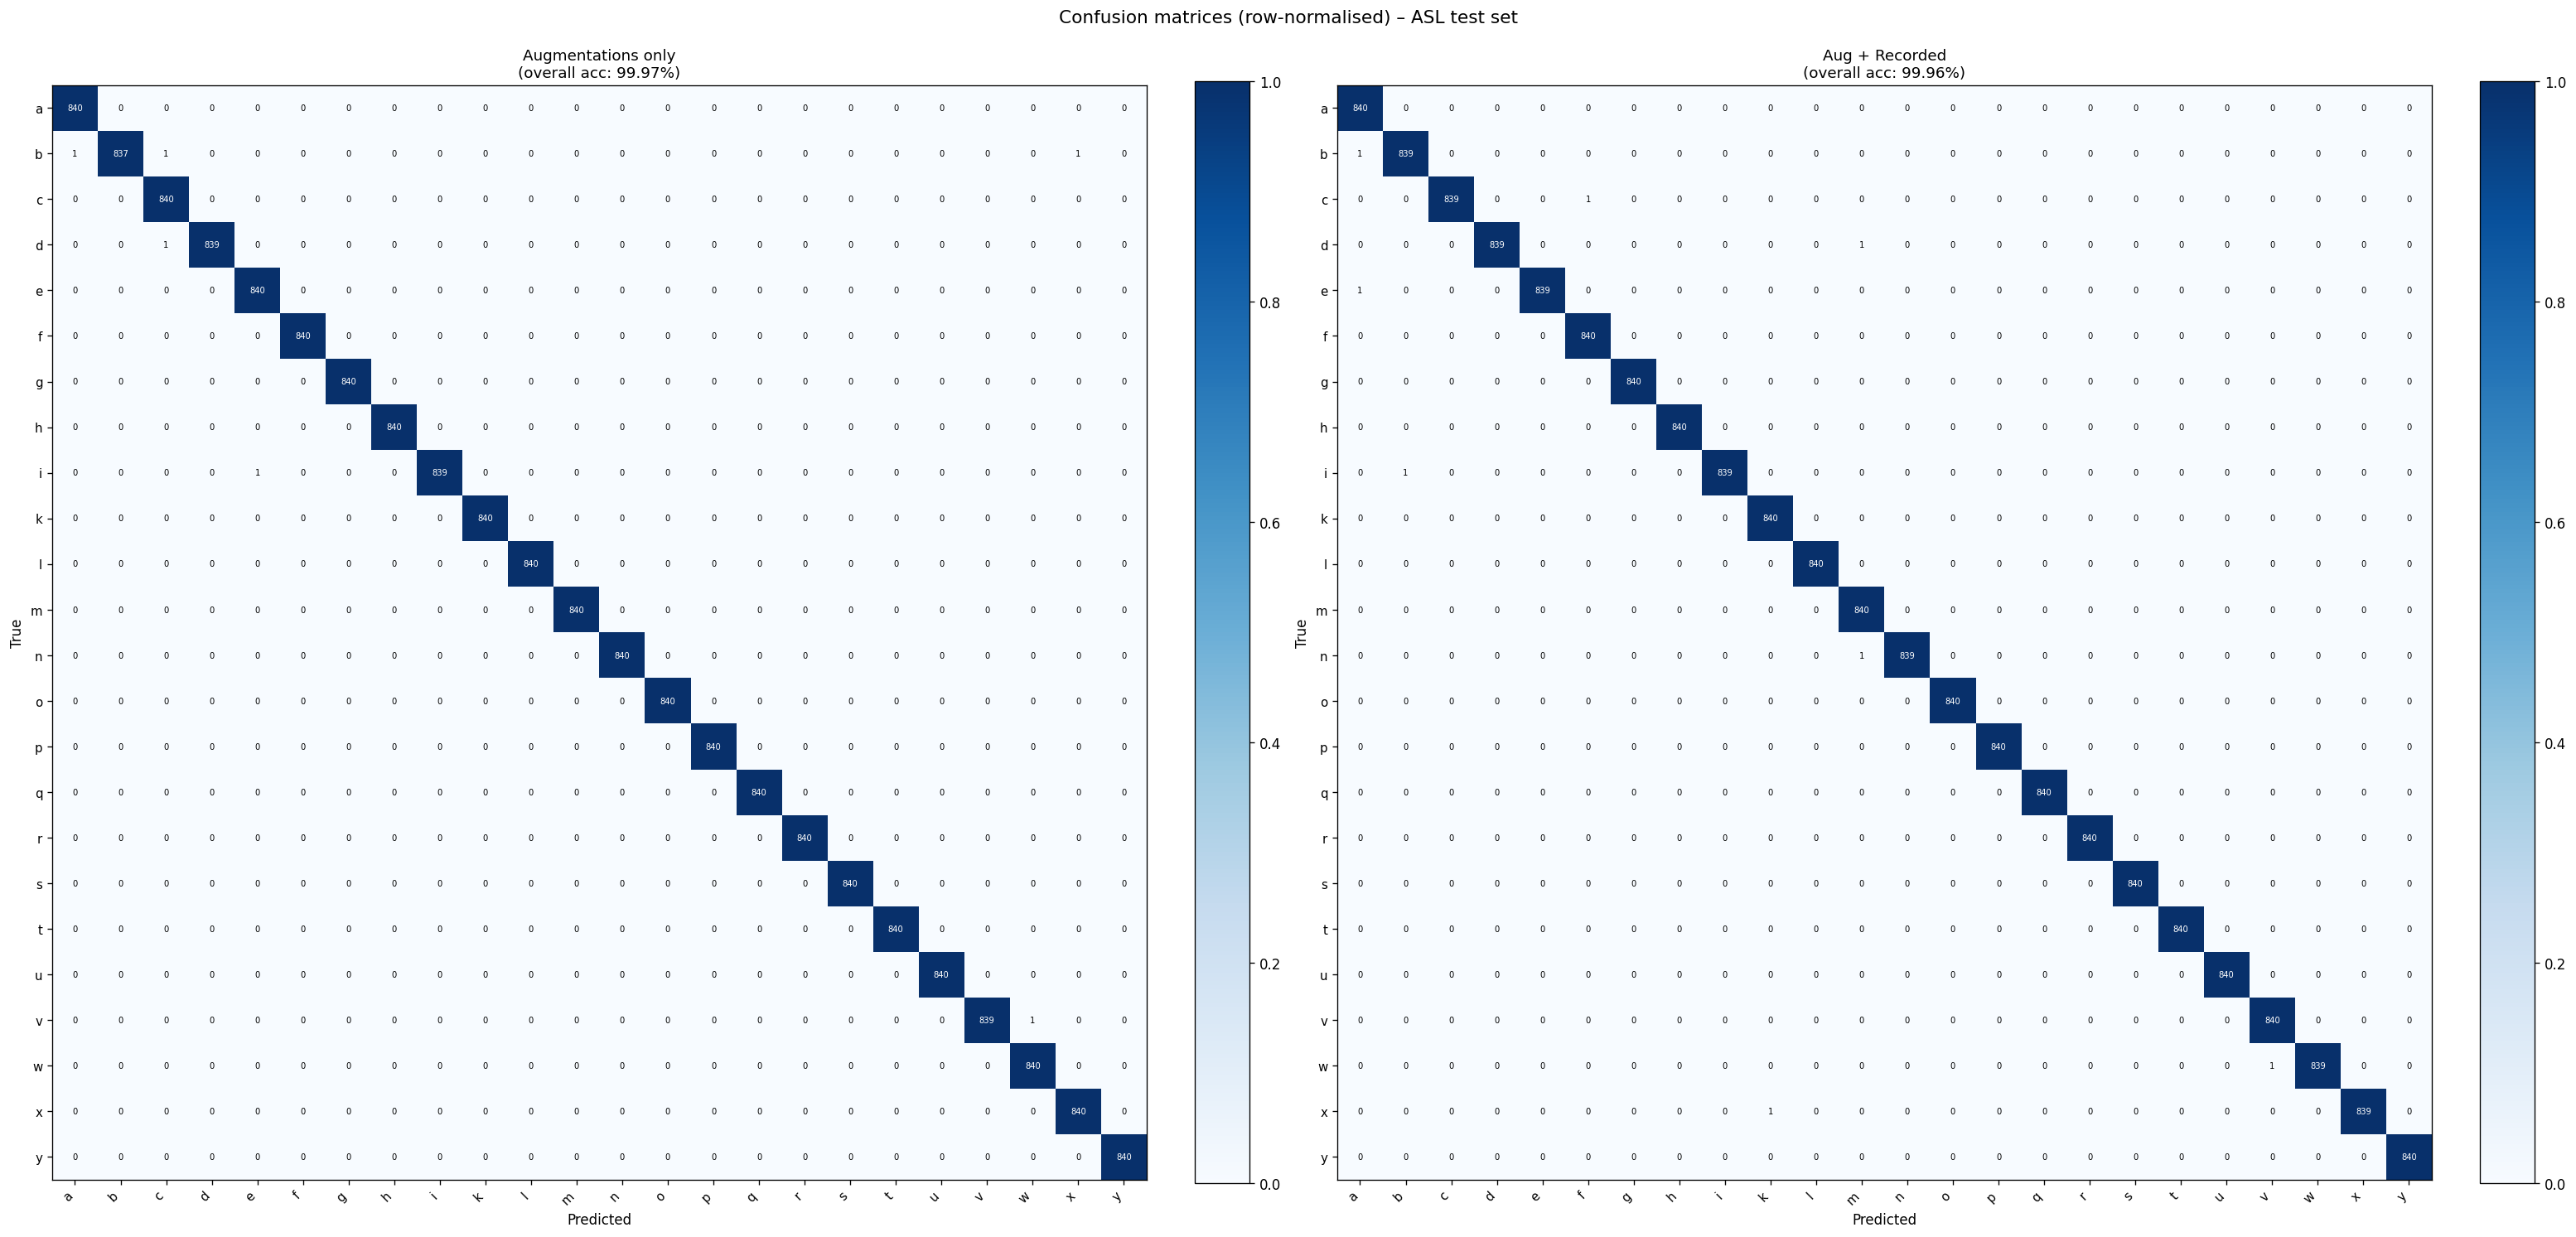
\includegraphics[width=\columnwidth]{confusion_matrices.png}
		\caption{Row-normalised confusion matrices on the ASL-DVS test set for the \textit{Aug only} (left, 99.97\%) and \textit{Aug + Recorded} (right, 99.98\%) models. Both matrices are near-perfect diagonals; minor off-diagonal mass appears on visually similar letter pairs.}
		\label{fig:confusion}
	\end{figure}

	\subsection{Discussion}

	The results confirm that accumulated two-channel event frames with a standard lightweight CNN backbone match or exceed specialised neuromorphic architectures on the ASL-DVS benchmark, while remaining simple to train and deploy on CPU hardware. The domain-bridging augmentations (vertical flip, rotation, scale jitter, contrast scaling, event dropout) are central to this result: without them, the DAVIS240C-trained model would not be expected to transfer to the GenX320's different noise profile and aspect ratio.

	The marginal gain from adding GenX320 recorded data (0.01 pp on the clean test set) is expected given that the test set is itself from the DAVIS240C and does not exercise the sensor-specific characteristics the recorded data was collected to address. The more meaningful evaluation — live inference accuracy on the GenX320 — is outside the scope of quantitative measurement here but is the primary motivation for collecting and oversampling the recorded data. The aspect-ratio mismatch between the square GenX320 FOV and the 4:3 DAVIS240C training data remains a source of potential performance degradation that collecting a larger, labelled GenX320 dataset would fully resolve.

	% ============================================================
	\section{Conclusion and Future Work}
	\label{sec:conclusion}
	% ============================================================

	This paper presented a complete machine vision system for event-based ASL gesture recognition using the Prophesee GenX320 event camera. A modified MobileNetV3-Small with a two-channel event input achieves 99.97\% accuracy on the ASL-DVS test set when trained with domain-bridging augmentations, and 99.98\% when ${\sim}$1,500 GenX320-recorded samples are additionally included with oversampling — both well above the ${\sim}91\%$ of prior graph-based methods on the same dataset. The \textit{accumulate\_then\_resize} domain adaptation strategy bridges the resolution and aspect-ratio gap between the DAVIS240C training sensor and the GenX320 deployment sensor, with a shared \texttt{PreprocessConfig} contract guaranteeing consistent preprocessing across training, evaluation, and live inference. Real-time inference is delivered via a Flask web dashboard with a streak-based confidence accumulation mechanism for temporal stability.

	The primary limitation is that quantitative evaluation is restricted to the clean ASL-DVS test set, which does not capture the full domain shift expected in live GenX320 deployment. The ~1,500 recorded GenX320 samples represent a promising start, but a larger, diverse labelled capture would be needed to measure and close the live-deployment performance gap. Additional improvements include dynamic gesture recognition using temporal models, INT8 quantisation for faster CPU inference, and multi-subject evaluation to assess robustness to signing style variation.

	\bibliographystyle{IEEEtran}
	\bibliography{machine_vision_report.bib}

\end{document}
